\documentclass[a4paper,10pt]{article}
\usepackage[utf8]{inputenc}
\usepackage[margin=1.5cm, bottom=2cm]{geometry}
\usepackage{fancyhdr}
\usepackage{enumitem}
\usepackage{xcolor}
\usepackage{makeidx}
\usepackage[most]{tcolorbox}
\newtcolorbox{osservazioni}{
  colback=gray!8,    % sfondo grigio chiaro
  colframe=white,      % nessun bordo
  arc=2mm,            % angoli smussati
  boxrule=0pt,        % spessore bordo 0
  fontupper=\footnotesize,
  left=2mm, right=2mm, top=2mm, bottom=2mm,
  before skip=7pt,   % niente spazio prima
  after skip=15pt     % niente spazio dopo
}
\newtcolorbox{osservazioni2}{
  colback=gray!8,    % sfondo grigio chiaro
  colframe=white,      % nessun bordo
  arc=2mm,            % angoli smussati
  boxrule=0pt,        % spessore bordo 0
  fontupper=\small,
  left=5mm, right=5mm, top=3mm, bottom=3mm,
  before skip=0pt,   % niente spazio prima
  after skip=30pt     % niente spazio dopo
}
\pagestyle{fancy}
\usepackage{tikz}
\usetikzlibrary{automata, positioning}
\pagestyle{fancy}

\usepackage{makeidx}

%%%%%%%%%%%%%%%%%%%
\newcommand{\EsercitazioneNum}{04}
\newcommand{\Data}{16/10/2025}
\newcommand{\DocType}{Esercitazione} % o "Eserciziario"
\newcommand{\FullTitle}{\DocType\ \EsercitazioneNum}

\newcommand{\Header}{
\noindent
  \small \textbf{Computabilità, Complessità e Logica - a.a. 2025/26} \hfill \textbf{\FullTitle} \\[0.2cm]
  \scriptsize Matteo Liotta, \texttt{matteo.liotta@studenti.units.it} \hfill \Data \\[0.2cm]
  \noindent\makebox[\linewidth]{\rule{\linewidth}{0.4pt}} \\[0.3cm]}

\newcommand{\NewPageHeader}{
  \vfill
  \noindent\makebox[\linewidth]{\rule{\linewidth}{0.4pt}}
  \newpage
  {\Header}
}
%%%%%%%%%%%%%%%%%%%

% Numero di pagina in basso al centro
\fancyhf{}
\fancyfoot[C] \thepage
\renewcommand{\footrulewidth}{0pt} % niente linea in basso
\renewcommand{\headrulewidth}{0pt} % niente linea in alto

\begin{document}

\footnotesize  % font generale più piccolo
\Header\\[0.7cm]


%%%%%%%%%%%%%%%% FOGLIO 5
%% INDEX
\addcontentsline{toc}{section}{Esercitazione 05: \textit{Automi a Pila e Linguaggi liberi dal contesto}} 
%%
\noindent\Large \textbf{Esercitazione 05}: \textit{Automi a Pila e Linguaggi liberi dal contesto}
\begin{osservazioni}
    \textbf{\textit{Nota}}. Sono indicati in \textcolor{blue}{\textit{blu}} gli esercizi che non saranno trattati durante l'esercitazione, bensì lasciati come strumento aggiuntivo di esercitazione individuale. Resta comunque assoluta disponibilità per la loro risoluzione negli incontri successivi, qualora necessario.
\end{osservazioni}

{\normalsize
\begin{itemize}[label=, leftmargin=0pt]

    \item \underline{\textit{\textbf{Costruzione di automi a pila da linguaggio context free}}}
    
    %% INDEX
    \addcontentsline{toc}{subsection}{Esercizio 37.} 
    %%
    \item \textbf{Esercizio 37. (*)}\\ 
    Sia $L$ linguaggio regolare su $\Sigma=\{a,b\}$, tale per cui 
    {\begin{center}
        $L = \{ w\in \Sigma^* \mid w=w_1.a.w_2,\quad w_1, w_2\in \Sigma^+\}$\\
    \end{center}}
    Si rappresenti l'automa a pila che riconosce tale linguaggio.\\

    \begin{osservazioni}
    \underline{\textit{Soluzione.}}

    Il linguaggio in questione si riconosce essere regolare, in quanto non sono espressi particolari sulla definizione di $w_1,w_2 \in \Sigma^+ $. Non c'è necessità alcuna di utilizzare la pila, quindi le transizioni che considereremo saranno solo della forma, $\forall\sigma\in\Sigma$:

    {
    \small
    \begin{center}
    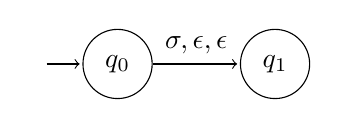
\begin{tikzpicture}[shorten >=1pt, node distance=2cm, on grid, auto]
        \node[state, initial, initial text=] (q0)   {$q_0$};
        \node[state] (q1) [right=of q0] {$q_1$};

        
        \path[->]
        (q0) edge  node {$\sigma, \epsilon, \epsilon$} (q1);
         
    \end{tikzpicture}
    \end{center}
    }
    Non sono specificati elementi da estrarre dalla pila, né elemeni da inserire. Considerando dapprima il caso in cui $w_1,w_2\in \Sigma^*$, la soluzione coincide con un automa che ammette tramite loop la scrittura di qualsiasi simbolo in ambo i nodi, collegati però da una transizione obbligata tramite $a$.


    {
    \small
    \begin{center}
    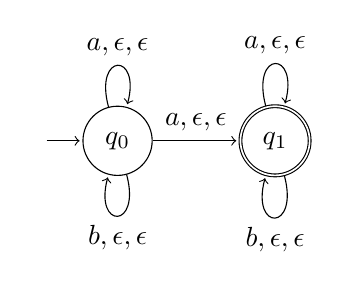
\begin{tikzpicture}[shorten >=1pt, node distance=2cm, on grid, auto]
        \node[state, initial, initial text=] (q0)   {$q_0$};
        \node[state, accepting] (q1) [right=of q0] {$q_1$};

        
        \path[->]
        (q0) edge [loop above] node {$a, \epsilon, \epsilon$} (q0)
        (q0) edge [loop below] node {$b, \epsilon, \epsilon$} (q0)
        edge  node {$a, \epsilon, \epsilon$} (q1)
        (q1) edge [loop above] node {$a, \epsilon, \epsilon$} (q1)
        (q1) edge [loop below] node {$b, \epsilon, \epsilon$} (q1);
         
    \end{tikzpicture}
    \end{center}
    }
    Per attenersi ad $L$, però, dobbiamo considerare parole in $\Sigma^+$: questo ci obbliga alla lettura di almeno un simbolo semplice, $a$ o $b$. Possiamo concludere allora obbligando a tale lettura.  

      {
    \small
    \begin{center}
    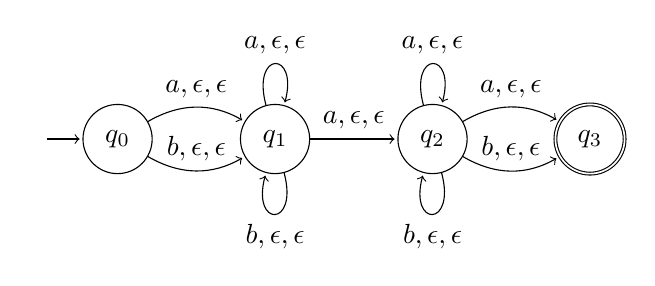
\begin{tikzpicture}[shorten >=1pt, node distance=2cm, on grid, auto]
        \node[state, initial, initial text=] (q0)   {$q_0$};
        \node[state] (q1) [right=of q0] {$q_1$};
        \node[state] (q2) [right=of q1] {$q_2$};
        \node[state, accepting] (q3) [right=of q2] {$q_3$};


        
        \path[->]
        (q1) edge [loop above] node {$a, \epsilon, \epsilon$} (q1)
        (q1) edge [loop below] node {$b, \epsilon, \epsilon$} (q1)
        edge  node {$a, \epsilon, \epsilon$} (q2)
        (q2) edge [loop above] node {$a, \epsilon, \epsilon$} (q2)
        (q2) edge [loop below] node {$b, \epsilon, \epsilon$} (q2)
        
        (q2) edge [bend right] node {$b, \epsilon, \epsilon$} (q3)
        (q2) edge [bend left] node {$a, \epsilon, \epsilon$} (q3)

        (q0) edge [bend right] node {$b, \epsilon, \epsilon$} (q1)
        (q0) edge [bend left] node {$a, \epsilon, \epsilon$} (q1);
         
    \end{tikzpicture}
    \end{center}
    }
    \end{osservazioni}


    
    %% INDEX
    \addcontentsline{toc}{subsection}{Esercizio 38.} 
    %%
    \item \textbf{Esercizio 38. (**)}\\ 
    Sia $L$ linguaggio c.f. su $\Sigma=\{a,b\}$, tale per cui 
    {\begin{center}
        $L = \{ w\in \Sigma^* \mid w=a^nb^n,\quad n\geq1\}$\\
    \end{center}}
    Si rappresenti l'automa a pila che riconosce tale linguaggio.

\begin{osservazioni}
    \underline{\textit{Soluzione.}}\\
    L'idea alla base della risoluzione è quella di usufruire della \textit{pila} per mantenere una memoria del numero di elementi di $a$ che sono stati letti prima del primo $b$. 
\end{osservazioni}
    
\NewPageHeader

\begin{osservazioni}
    A tal proposito l'idea è di inserire in pila un simbolo "$A$" ad ogni lettura di $a$, seguito da una estrazione di $A$ ad ogni lettura di $b$. È così possibile avere la certezza di aver inserito un numero di $b$ pari al numero di $a$, in un ordine $a^nb^n$ vincolato dalle transizioni stesse:

    
      {
    \small
    \begin{center}
    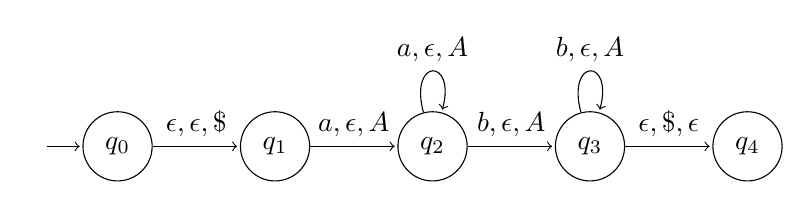
\begin{tikzpicture}[shorten >=1pt, node distance=2cm, on grid, auto]
        \node[state, initial, initial text=] (q0)   {$q_0$};
        \node[state] (q1) [right=of q0] {$q_1$};
        \node[state] (q2) [right=of q1] {$q_2$};
        \node[state] (q3) [right=of q2] {$q_3$};
        \node[state] (q4) [right=of q3] {$q_4$};


        
        \path[->]
        (q0) edge node {$\epsilon, \epsilon, \$ $} (q1)
        (q1) edge node {$a, \epsilon, A$} (q2)
        (q2) edge node {$b, \epsilon, A$} (q3)
        edge [loop above] node {$a, \epsilon, A$} (q2)
        (q3) edge [loop above] node {$b, \epsilon, A$} (q3)
        (q3) edge node {$\epsilon, \$, \epsilon$} (q4);
        
         
    \end{tikzpicture}
    \end{center}
    }
    
\end{osservazioni}

    %% INDEX
    \addcontentsline{toc}{subsection}{Esercizio 39.} 
    %%
    \textcolor{black}{\item \textbf{Esercizio 39. (**)}\\ }
    Sia $L$ linguaggio c.f. su $\Sigma=\{a,b\}$, tale per cui 
    {\begin{center}
        $L = \{ w\in \Sigma^* \mid w=a^nb^{2n},\quad n\geq 1\}$\\
    \end{center}} 
    Si rappresenti l'automa a pila che riconosce tale linguaggio.

\begin{osservazioni}
    \underline{\textit{Soluzione.}}\\
    La soluzione è analoga al caso precente. Si noti però che in questo caso, dal momento che ogni $b$ deve corrispondere a due $a$, è necessario leggere due simboli $A$ per inserire una b. Possiamo a tal proposito inseirire 2 simboli di A in una singola lettura sfruttando l'epsilon transizione.

  
      {
    \small
    \begin{center}
    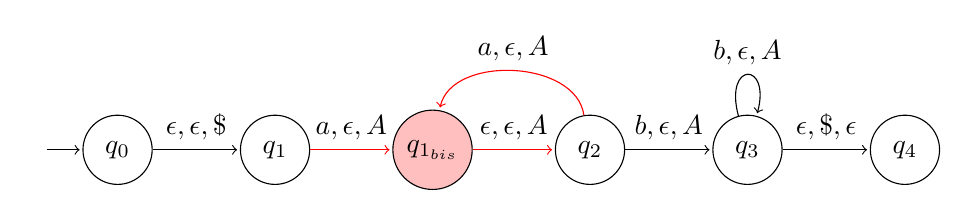
\begin{tikzpicture}[shorten >=1pt, node distance=2cm, on grid, auto]
        \node[state, initial, initial text=] (q0)   {$q_0$};
        \node[state] (q1) [right=of q0] {$q_1$};
        \node[state] (qA) [right=of q1, fill=red!25] {$q_{1_{bis}}$};
        \node[state] (q2) [right=of qA] {$q_2$};
        \node[state] (q3) [right=of q2] {$q_3$};
        \node[state] (q4) [right=of q3] {$q_4$};


        
        \path[->]
        (q0) edge node {$\epsilon, \epsilon, \$ $} (q1)
        (q1) edge [draw=red] node {$a, \epsilon, A$} (qA)
        (qA) edge [draw=red] node {$\epsilon, \epsilon, A$} (q2)
        (q2) edge node {$b, \epsilon, A$} (q3)
        edge [above, bend right=80, draw = red] node {$a, \epsilon, A$} (qA)
        (q3) edge [loop above] node {$b, \epsilon, A$} (q3)
        (q3) edge node {$\epsilon, \$, \epsilon$} (q4);
        
         
    \end{tikzpicture}
    \end{center}
    }
    In futuro potremo intendere la scrittura della transizione $a,\epsilon,AA$ come di questa forma (rosso), indicata così per brevità.
\end{osservazioni}

    %% INDEX
    \addcontentsline{toc}{subsection}{Esercizio 40.} 
    %%
    \textcolor{black}{\item \textbf{Esercizio 40. (*)}\\ }
    Sia $L$ linguaggio c.f. su $\Sigma=\{0,1\}$, tale per cui 

    {
    \small
    \begin{center}
    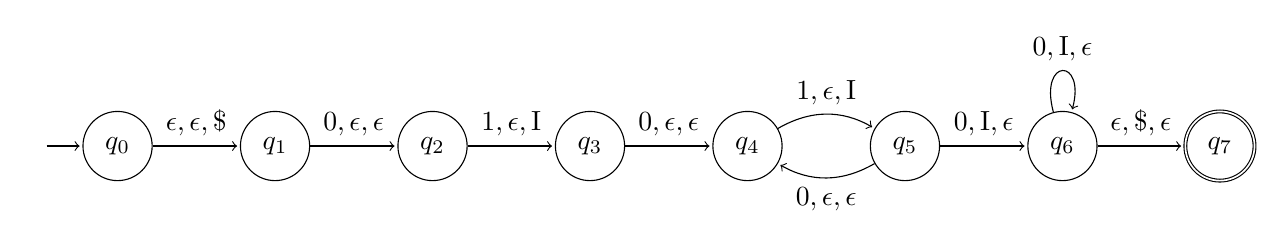
\begin{tikzpicture}[shorten >=1pt, node distance=2cm, on grid, auto]
        \node[state, initial, initial text=] (q0)   {$q_0$};
        \node[state] (q1) [right=of q0] {$q_1$};
        \node[state] (q2) [right=of q1] {$q_2$};
        \node[state] (q3) [right=of q2] {$q_3$};
        \node[state] (q4) [right=of q3] {$q_4$};
        \node[state] (q5) [right=of q4] {$q_5$};
        \node[state] (q6) [right=of q5] {$q_6$};
        \node[state, accepting] (q7) [right=of q6] {$q_7$};




        
        \path[->]
        (q0) edge  node {$\epsilon, \epsilon, \$$} (q1)
        (q1) edge node {$0, \epsilon, \epsilon$} (q2)
        (q2) edge node {$1,\epsilon, \text{I}$} (q3)
        (q3) edge node {$0,\epsilon, \epsilon$} (q4)
        (q4) edge [bend left] node {$1,\epsilon, \text{I}$} (q5)
        (q5) edge [bend left] node {$0,\epsilon, \epsilon$} (q4)
        (q5) edge node {$0, \text{I}, \epsilon$} (q6)
        (q6) edge [loop above] node {$0, \text{I}, \epsilon$} (q6)
        (q6) edge node {$\epsilon,\$, \epsilon$} (q7);
             
            
    \end{tikzpicture}
    \end{center}
    }
    
    Si individui il $L$ linguaggio riconosciuto dall'automa.

\begin{osservazioni}
    \underline{\textit{Soluzione.}}\\
    Dapprima si simuli la lettura e l'inserimento in stack:
    \begin{enumerate}
        \item Situazione iniziale con\\ \texttt{Stack: [] }
        \item \texttt{Letto: $\epsilon$} \texttt{Stack: [\$] }
        \item \texttt{Letto: 0} \texttt{Stack: [\$] }
        \item \texttt{Letto: 1} \texttt{Stack: [\$,I] }
        \item \texttt{Letto: 0} \texttt{Stack: [\$,I] }
        \item Loop di letture che inseriscono una $I$ ad ogni lettura di un $1$.
    \end{enumerate}
    Si osserva come il all'inizio le parole sono della forma $0101$ e possono essere seguite da $(01)$ per un numero arbitrario di volte. Alla fine, devono essere letti tanti zero quanti simboli $I$ sono stati inseriti. Poiché inserito uno ad ogni lettura di 1, allora il loop deve essere eseguito in numero uguale al numero di 1 prima inseriti. Dunque

    $$w\in L \Leftrightarrow w=0101(01)^n0^{n+2}, \quad n\ge0 $$

    
\end{osservazioni}

\NewPageHeader

    %% INDEX
    \addcontentsline{toc}{subsection}{Esercizio 41.} 
    %%
    \item \textcolor{blue}{\textbf{Esercizio 41. (***)}}\\ 
    Sia $L$ linguaggio c.f. su $\Sigma=\{a,b\}$, tale per cui 
    {\begin{center}
        $L = \{ w\in \Sigma^* \mid \#a = \#b \text{\ in\ }w \}$\\
    \end{center}}
    Si rappresenti l'automa a pila che riconosce tale linguaggio.\\

    \begin{osservazioni}
        \underline{\textit{Soluzione.}}\\
        A differenza di altri esercizi, qui vediamo come non sia imposto alcun ordinamento interno alle parole accettate dall'automa. Partiamo da alcune considerazioni chiave prima di passare alla risoluzione. 

        \begin{itemize}
            \item Qualsiasi sia la condizione iniziale dell'automa, sappiamo che potremo leggere un simbolo di $\Sigma$, $a$ o $b$. 
            \item Se così, possiamo aspettarci che l'automa abbia almeno una seguente forma iniziale:

            {
            \small
            \begin{center}
        	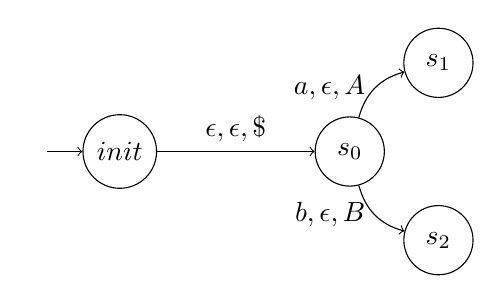
\begin{tikzpicture}
                \node[state, initial, initial text=] (init) {$init$};
        		\node[state] (s0) [right=2of init] {$s_0$};
        		\node[state] (s1) [above right=0.7of s0] {$s_1$};
        		\node[state] (s2) [below right=0.7of s0] {$s_2$};
        		
        		\path[->] 
                (init) edge[above] node{$\epsilon,\epsilon,\$$} (s0)
                (s0) edge[bend left, left] node {$a,\epsilon,A$} (s1)
                (s0) edge[bend right, left] node {$b,\epsilon,B$} (s2);
            \end{tikzpicture}
            \end{center}
            }

            \item Analizzando il precedente, se leggiamo $a$, la pila conterrà a questo punto 
            {
            \begin{center}
                \texttt{[\$,A]}
            \end{center}
            }
            oppure prendendo l'arco etichettato con $b$ 
            {
            \begin{center}
                \texttt{[\$,B]}
            \end{center}
            }
            Come possiamo interpretare questa informazione? Avendo \texttt{[\$, A]} stiamo mantendendo implicitamente l'informazione che \textit{abbiamo letto \textbf{una $a$ in più di $b$}}.
    
        \end{itemize}
    Queste considerazioni sono essenziali in quanto sono la chiave per la generalizzazione. Possiamo aggiungere altri punti, come il significato che ci aspettiamo di poter attribuire alla pila, sia comportamenti che da essa ci aspettiamo:
    \begin{enumerate}
        \item Sappiamo se la pila è vuota tramite il carattere \$ al suo interno
        \item Non vogliamo che simboli siano mischiati all'interno della pila, poiché vogliamo che la pila mantenga espressa la situazione di \textbf{debito} che ha la parola letta fino alla $i$-esima lettera nei confronti di termini $a$ o $b$. 
        Inoltre, ci aspettiamo -come visto sopra- di poter costruire due zone simmetriche rispetto a $s_0$ in cui mantenere il debito attivo rispettivamente nei confronti di $a$ o di $b$. 
        \item Ci aspettiamo che il debito di $a$ o $b$ si possa saldare \textbf{completamente}, garantendo la possibilità di avere un debito nella stessa lettera o nell'opposta. Se il debito si sposta da $a$ a $b$ o viceversa, ci aspettiamo di poterlo capire tramite la lettura corrente e la situazione di pila vuota (con \$): la pila vuota testimonia l'assenza di debito e quindi è la chiave per lo spostamento all'altra porzione.
    \end{enumerate}
    Con questo chiaro, possiamo considerare\textit{ ad alto livello }l'automa:
    \begin{enumerate}
        \item Partendo da $s_0$ la pila contiene \texttt{[\$]}
        \item Supponiamo sia letta la prima parola di $w\in L$ e sia tale lettera $a$.
        \item La situazione nella pila cambia, portandola a \texttt{[\$,A]}
        \item A questo punto ci aspettiamo di poter incrementare il debito tramite un loop che continua a leggere $a$ e scrivere $A$ in pila: \texttt{[\$, A, A, ..., A]}
        \item In questa fase, l'eventuale lettura di termini $b$ ci permette di saldare \textbf{di una lettura} (quindi di un simbolo in pila) il debito. Ci si aspetta di poter ammettere dunque non solo transizioni che aumentino il debito, ma che lo saldino:
        $$\delta(s_1,b,A,\epsilon)\rightarrow s_1$$
        \item Possiamo aspettarci anche l'eventualità che il numero di $b$ sia sufficiente, al passo $i$, da coprire completamente il numero di $a$ inserito, ritornando a una situazione di lettura pari, con conseguente pila nuovamente vuota: \texttt{[\$]}. 
        \item La lettura di altre $a$ incrementerebbe il debito -quindi la situazione è già coperta dalla considerazioni precedenti. Invece, la lettura di $b$ in $s_1$, dato che la pila è vuota, dovrebbe portarci a considerare un debito sulle $b$. Abbiamo una zona che gestisce tale debito: il nodo $s_2$. Possiamo allora effettuare una transizione del tipo:
        $$ \delta(s_1,b,\$,\$) \rightarrow s_3;\quad  
           \delta(s_3,\epsilon,\$,B) \rightarrow s_2$$
        Dove vediamo che se la pila è vuota (necessario prendere e reinserire \$) e viene letta una $b$ invece che una $a$, allora si incrementa il debito con $B$.
    \end{enumerate}
    \end{osservazioni}

\NewPageHeader

\begin{osservazioni}
    Con questo chiaro, ricordando la simmetria dell'automa, possiamo costruire:
{
            \small
            \begin{center}
        	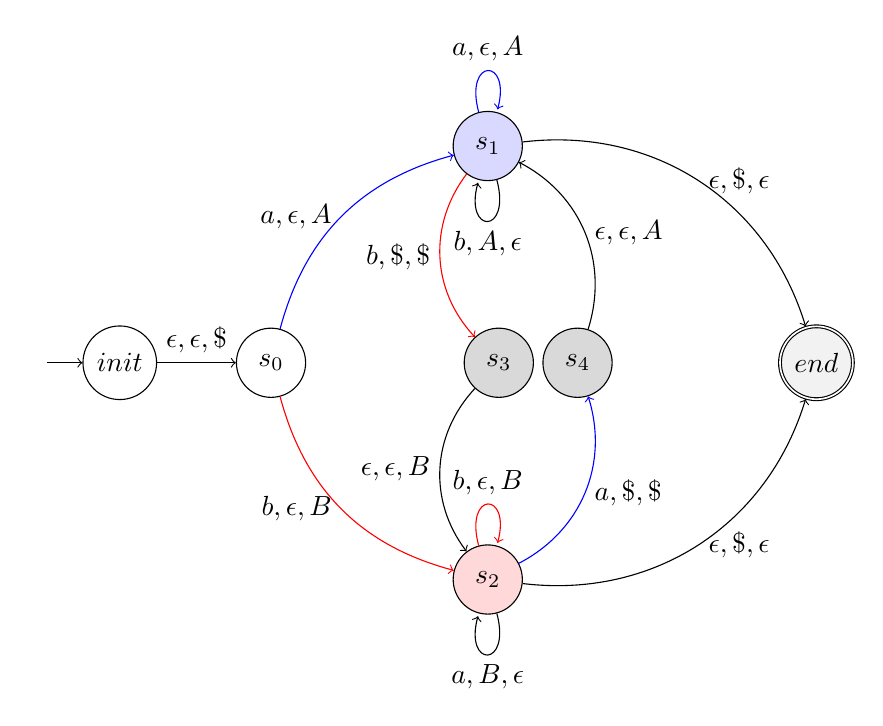
\begin{tikzpicture}
                \node[state, initial, initial text=] (init) {$init$};
        		\node[state] (s0) [right=1of init] {$s_0$};
        		\node[state] (s1) [above right=3of s0, fill=blue!15] {$s_1$};
        		\node[state] (s2) [below right=3of s0,fill=red!15] {$s_2$};
                \node[state] (s3) [right=2of s0, fill=black!15] {$s_3$};
                \node[state] (s4) [right=3of s0, fill=black!15] {$s_4$};
                \node[state, accepting] (end) [right=6of s0, fill=black!5] {$end$};


        		
        		\path[->] 
                (init) edge[above] node{$\epsilon,\epsilon,\$$} (s0)
                (s0) edge[bend left, left, draw=blue] node {$a,\epsilon,A$} (s1)
                (s0) edge[bend right, left, draw=red] node {$b,\epsilon,B$} (s2)

                % nodi per gestire il saldo senza problemi
                (s1) edge[loop above, above, draw=blue] node {$a,\epsilon,A$} (s1)
                (s2) edge[loop above, above,draw=red] node {$b,\epsilon,B$} (s2)
                (s1) edge[loop below, below, draw=black] node {$b,A,\epsilon$} (s1)
                (s2) edge[loop below, below, draw=black] node {$a,B,\epsilon$} (s2)

                % gestione del saldo con pila vuota
                (s1) edge[bend right=40, left, draw=red] node {$b, \$, \$$} (s3)
                (s3) edge[bend right=40, left, draw=black] node {$\epsilon, \epsilon, B$} (s2)

                (s2) edge[bend right=40, right, draw=blue] node {$a, \$, \$$} (s4)
                (s4) edge[bend right=40, right, draw=black] node {$\epsilon, \epsilon, A$} (s1)

                %accept
                (s2) edge[bend right=40, right] node {$\epsilon,\$,\epsilon$} (end)
                (s1) edge[bend left=40, right] node {$\epsilon,\$,\epsilon$} (end);
                
                
                
                
                
            \end{tikzpicture}
            \end{center}
            }
    
\end{osservazioni}
    
\end{itemize}
}
\vfill
\noindent\makebox[\linewidth]{\rule{\linewidth}{0.1pt}}
\end{document}
